\tikzset{every picture/.style={line width=0.75pt}} %set default line width to 0.75pt        

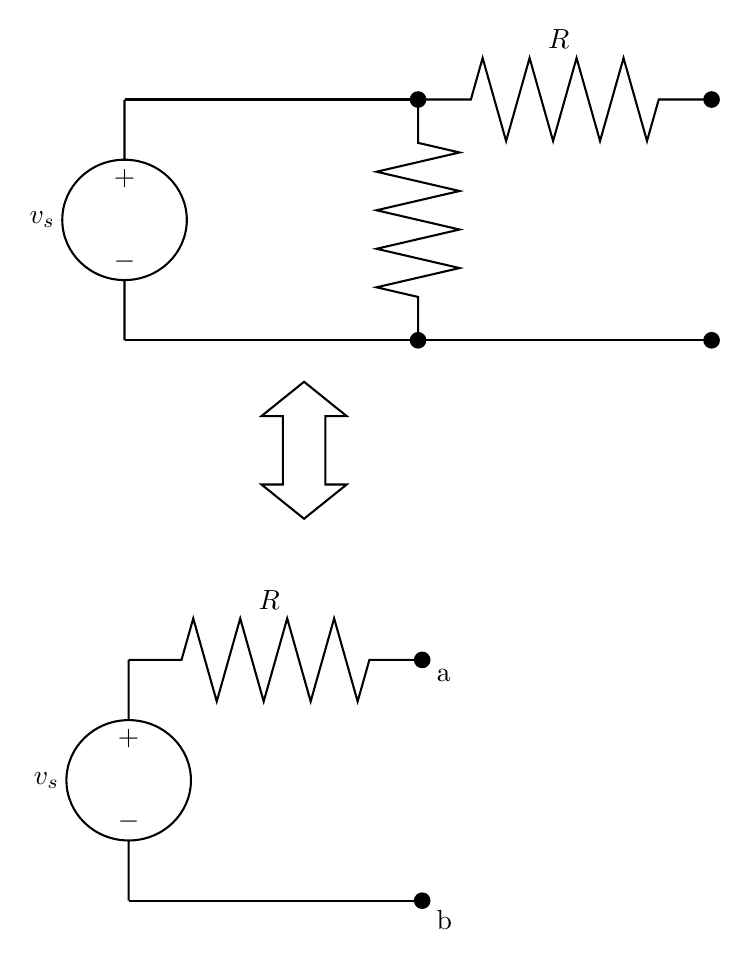
\begin{tikzpicture}[x=0.75pt,y=0.75pt,yscale=-1,xscale=1]
%uncomment if require: \path (0,642); %set diagram left start at 0, and has height of 642

%Shape: Output [id:dp4761018043956171] 
\draw   (254,86) .. controls (270.57,86) and (284,98.98) .. (284,115) .. controls (284,131.02) and (270.57,144) .. (254,144) .. controls (237.43,144) and (224,131.02) .. (224,115) .. controls (224,98.98) and (237.43,86) .. (254,86) -- cycle (254,57) -- (254,86) (254,173) -- (254,144) ;
%Straight Lines [id:da18038673316668685] 
\draw    (395.42,173) -- (254,173) ;
%Shape: Resistor [id:dp49094225036149086] 
\draw   (395.42,57) -- (420.88,57) -- (426.53,37) -- (437.85,77) -- (449.16,37) -- (460.48,77) -- (471.79,37) -- (483.1,77) -- (494.42,37) -- (505.73,77) -- (511.39,57) -- (536.84,57) ;
%Shape: Circle [id:dp7252316282946523] 
\draw  [fill={rgb, 255:red, 0; green, 0; blue, 0 }  ,fill opacity=1 ] (391.92,57) .. controls (391.92,55.07) and (393.49,53.5) .. (395.42,53.5) .. controls (397.35,53.5) and (398.92,55.07) .. (398.92,57) .. controls (398.92,58.93) and (397.35,60.5) .. (395.42,60.5) .. controls (393.49,60.5) and (391.92,58.93) .. (391.92,57) -- cycle ;
%Shape: Circle [id:dp7082112398028335] 
\draw  [fill={rgb, 255:red, 0; green, 0; blue, 0 }  ,fill opacity=1 ] (391.92,173) .. controls (391.92,171.07) and (393.49,169.5) .. (395.42,169.5) .. controls (397.35,169.5) and (398.92,171.07) .. (398.92,173) .. controls (398.92,174.93) and (397.35,176.5) .. (395.42,176.5) .. controls (393.49,176.5) and (391.92,174.93) .. (391.92,173) -- cycle ;
%Shape: Output [id:dp6368500887380681] 
\draw   (256,356) .. controls (272.57,356) and (286,368.98) .. (286,385) .. controls (286,401.02) and (272.57,414) .. (256,414) .. controls (239.43,414) and (226,401.02) .. (226,385) .. controls (226,368.98) and (239.43,356) .. (256,356) -- cycle (256,327) -- (256,356) (256,443) -- (256,414) ;
%Straight Lines [id:da25378864334436835] 
\draw    (397.42,443) -- (256,443) ;
%Shape: Resistor [id:dp10671543731782762] 
\draw   (256,327) -- (281.46,327) -- (287.11,307) -- (298.43,347) -- (309.74,307) -- (321.05,347) -- (332.37,307) -- (343.68,347) -- (354.99,307) -- (366.31,347) -- (371.97,327) -- (397.42,327) ;
%Shape: Circle [id:dp522496327022093] 
\draw  [fill={rgb, 255:red, 0; green, 0; blue, 0 }  ,fill opacity=1 ] (393.92,327) .. controls (393.92,325.07) and (395.49,323.5) .. (397.42,323.5) .. controls (399.35,323.5) and (400.92,325.07) .. (400.92,327) .. controls (400.92,328.93) and (399.35,330.5) .. (397.42,330.5) .. controls (395.49,330.5) and (393.92,328.93) .. (393.92,327) -- cycle ;
%Shape: Circle [id:dp8014445694731585] 
\draw  [fill={rgb, 255:red, 0; green, 0; blue, 0 }  ,fill opacity=1 ] (393.92,443) .. controls (393.92,441.07) and (395.49,439.5) .. (397.42,439.5) .. controls (399.35,439.5) and (400.92,441.07) .. (400.92,443) .. controls (400.92,444.93) and (399.35,446.5) .. (397.42,446.5) .. controls (395.49,446.5) and (393.92,444.93) .. (393.92,443) -- cycle ;
%Straight Lines [id:da18260678273306796] 
\draw    (395.42,57) -- (254,57) ;
%Shape: Resistor [id:dp684354118396199] 
\draw   (395.42,57) -- (395.42,77.88) -- (415.42,82.52) -- (375.42,91.8) -- (415.42,101.08) -- (375.42,110.36) -- (415.42,119.64) -- (375.42,128.92) -- (415.42,138.2) -- (375.42,147.48) -- (395.42,152.12) -- (395.42,173) ;
%Straight Lines [id:da8845127840871825] 
\draw    (536.84,173) -- (395.42,173) ;
%Shape: Circle [id:dp9978288916988585] 
\draw  [fill={rgb, 255:red, 0; green, 0; blue, 0 }  ,fill opacity=1 ] (533.34,57) .. controls (533.34,55.07) and (534.91,53.5) .. (536.84,53.5) .. controls (538.78,53.5) and (540.34,55.07) .. (540.34,57) .. controls (540.34,58.93) and (538.78,60.5) .. (536.84,60.5) .. controls (534.91,60.5) and (533.34,58.93) .. (533.34,57) -- cycle ;
%Shape: Circle [id:dp9681776211546007] 
\draw  [fill={rgb, 255:red, 0; green, 0; blue, 0 }  ,fill opacity=1 ] (533.34,173) .. controls (533.34,171.07) and (534.91,169.5) .. (536.84,169.5) .. controls (538.78,169.5) and (540.34,171.07) .. (540.34,173) .. controls (540.34,174.93) and (538.78,176.5) .. (536.84,176.5) .. controls (534.91,176.5) and (533.34,174.93) .. (533.34,173) -- cycle ;
%Up Down Arrow [id:dp03182684902749244] 
\draw   (320,209.5) -- (340.5,193) -- (361,209.5) -- (350.75,209.5) -- (350.75,242.5) -- (361,242.5) -- (340.5,259) -- (320,242.5) -- (330.25,242.5) -- (330.25,209.5) -- cycle ;

% Text Node
\draw (222,115) node [anchor=east] [inner sep=0.75pt]   [align=left] {$\displaystyle v_{s}$};
% Text Node
\draw (469.79,34) node [anchor=south east] [inner sep=0.75pt]   [align=left] {$\displaystyle R$};
% Text Node
\draw (254,89) node [anchor=north] [inner sep=0.75pt]   [align=left] {\begin{minipage}[lt]{8.68pt}\setlength\topsep{0pt}
\begin{center}
+
\end{center}

\end{minipage}};
% Text Node
\draw (254,141) node [anchor=south] [inner sep=0.75pt]   [align=left] {$\displaystyle -$};
% Text Node
\draw (224,385) node [anchor=east] [inner sep=0.75pt]   [align=left] {$\displaystyle v_{s}$};
% Text Node
\draw (330.37,304) node [anchor=south east] [inner sep=0.75pt]   [align=left] {$\displaystyle R$};
% Text Node
\draw (256,359) node [anchor=north] [inner sep=0.75pt]   [align=left] {\begin{minipage}[lt]{8.68pt}\setlength\topsep{0pt}
\begin{center}
+
\end{center}

\end{minipage}};
% Text Node
\draw (256,411) node [anchor=south] [inner sep=0.75pt]   [align=left] {$\displaystyle -$};
% Text Node
\draw (402.92,330) node [anchor=north west][inner sep=0.75pt]   [align=left] {a};
% Text Node
\draw (402.92,446) node [anchor=north west][inner sep=0.75pt]   [align=left] {b};


\end{tikzpicture}
